% Overleaf: pega este archivo como main.tex
% Sube a la raíz del proyecto Overleaf:
%   logo_uexternado.png
%   fig_roc.png, fig_pr.png, fig_coeficientes.png  (desde codigo/salidas/)
% Si existe un archivo output.pdf en el proyecto, bórralo o renómbralo.

\documentclass[11pt]{article}
\usepackage[utf8]{inputenc}
\usepackage[T1]{fontenc}
\usepackage[margin=2.5cm]{geometry}
\usepackage{booktabs}
\usepackage{graphicx}
\usepackage{hyperref}
\usepackage{enumitem}
\usepackage{parskip}
\usepackage{float}
\usepackage{amsmath}
\usepackage{url}

\hypersetup{
    colorlinks=true, linkcolor=black, urlcolor=black, citecolor=black,
    pdftitle={Riesgo de incumplimiento crediticio - Segunda entrega},
    pdfauthor={Isabella Pensamiento, Juan Angel Triana}
}

\setlist[itemize]{leftmargin=1.4em, itemsep=1pt, topsep=2pt}
\setlist[enumerate]{leftmargin=1.6em, itemsep=1pt, topsep=2pt}

\renewcommand{\tablename}{Tabla}
\renewcommand{\figurename}{Figura}

\newcommand{\incluirlogo}{%
  \IfFileExists{logo_uexternado.png}{%
    \includegraphics[width=6cm]{logo_uexternado.png}%
  }{%
    \vspace{2.5cm}{\small\textit{(Sube logo\_uexternado.png)}}%
  }%
}

\begin{document}

\begin{titlepage}
\centering
\incluirlogo
\vspace{0.7cm}

{\bfseries\large UNIVERSIDAD EXTERNADO DE COLOMBIA\par}
\vspace{2pt}
{\bfseries FACULTAD DE MATEMÁTICAS\par}
{PREGRADO EN CIENCIA DE DATOS\par}
\vspace{1.6cm}

\rule{\linewidth}{0.6pt}
\vspace{0.4cm}

{\Large\bfseries Riesgo de Incumplimiento Crediticio\par}
\vspace{0.3cm}
{\large Regresión Logística en el Contexto Latinoamericano\par}
\vspace{0.3cm}
{Segunda Entrega -- Proyecto Integrador\par}
\vspace{0.4cm}

\rule{\linewidth}{0.6pt}
\vspace{1.6cm}

{\large Isabella Pensamiento\par}
{\large Juan Angel Triana\par}
\vspace{0.8cm}

{\large Machine Learning I\par}
\vspace{0.3cm}
Profesora: Juliana De Mier
\vspace{2.5cm}

\vfill
{\bfseries Bogotá D.C. -- Colombia\par}
Octubre de 2026
\end{titlepage}

\section{Ajustes a la primera entrega}

Antes de modelar precisamos qué significa \texttt{mora}, en qué momento se haría la predicción y si \texttt{atraso}, \texttt{clasif\_sbs} y \texttt{score} pueden filtrar la respuesta. También reformulamos la pregunta hacia un objetivo predictivo, dejamos de tratar el 70\% de precision como regla de calidad y separamos los supuestos de la logística de las decisiones de limpieza. Eso se desarrolla en las secciones~2, 3, 6 y~8.

Al revisar los datos cambiamos algunas piezas del plan. La Tabla~\ref{tab:cambios} resume qué cambió y por qué. Mantenemos la línea base que predice siempre mora. El código está en el notebook que acompaña este informe y todas las cifras salen de ahí.

\begin{table}[H]
\centering
\caption{Cambios frente al plan de la primera entrega.}
\label{tab:cambios}
\small
\begin{tabular}{@{}p{2.2cm}p{4.2cm}p{6.8cm}@{}}
\toprule
\textbf{Tema} & \textbf{Primera entrega} & \textbf{Ahora y por qué} \\
\midrule
Modelos & Regresión logística, Ridge/Lasso, LDA y KNN & Logística, LDA, KNN y Naive Bayes. Ridge/Lasso y QDA quedan para la entrega final \\
Naive Bayes & Fuera de los principales, por suponer independencia & Sigue sin ser principal. Entra solo como contraste \\
Balanceo & Evaluar si conviene & Cinco opciones probadas. El AUC no mejora, así que entrenamos sin balancear \\
Imputación & Mediana & Mediana más indicador de faltante \\
Variables & 13 predictores & Escenario principal de 11, sin \texttt{atraso} ni \texttt{clasif\_sbs} \\
Métricas & AUC y meta de precision & AUC y PR-AUC. Sin metas fijas frente a la línea base \\
Pregunta & Qué características aumentan la probabilidad de mora & Qué tan bien puede predecirse el riesgo de mora \\
\bottomrule
\end{tabular}
\end{table}

\section{Pregunta, definición de \texttt{mora} y momento de predicción}

\textbf{Pregunta.} Buscamos responder: \textbf{¿qué tan bien puede predecirse el riesgo de mora de un cliente de crédito de consumo a partir de información financiera y socioeconómica disponible previamente?} Primero medimos qué tan bien se predice. Después leemos las variables, sin tratar los coeficientes como causas.

\textbf{Qué significa \texttt{mora}.} El autor habla de pagador al día o cliente moroso, pero no publica un diccionario de datos. Encontramos que \texttt{mora} no es lo mismo que tener atraso hoy: el 57,7\% de los clientes con \texttt{mora = 1} tiene \texttt{atraso = 0}, y el 27,2\% de los con \texttt{mora = 0} sí tiene días de atraso. Por eso usamos esta definición operativa:
\begin{quote}
\texttt{mora = 1} significa que el cliente aparece marcado como moroso en la base. \texttt{mora = 0} significa que aparece como pagador al día.
\end{quote}
Es un supuesto nuestro y lo dejamos como limitación. No afirmamos que sea mora actual ni mora en un periodo exacto, porque la fuente no lo permite.

\textbf{Momento de predicción.} Pensamos el modelo para cuando el banco evalúa al cliente. En ese momento conoce el perfil, el historial y el \texttt{score}, pero aún no sabe si quedará marcado como moroso. Como la base no trae fechas, esto también es un supuesto. Lo revisamos variable por variable.

\section{Revisión de variables y riesgo de fuga}

Para cada variable nos preguntamos qué mide, cuándo se observa, si el banco la tendría antes de saber la \texttt{mora} y si la mora pudo usarse para construirla. La Tabla~\ref{tab:variables} resume las decisiones. Los momentos son supuestos razonables a partir de la descripción del autor.

\begin{table}[H]
\centering
\caption{Revisión de variables (resumen).}
\label{tab:variables}
\small
\begin{tabular}{@{}lll@{}}
\toprule
\textbf{Variable} & \textbf{¿Disponible antes de la mora?} & \textbf{Decisión} \\
\midrule
Perfil (edad, ingreso, zona, etc.) & Sí & Se usan \\
\texttt{exp\_sf}, \texttt{linea\_sf}, \texttt{deuda\_sf} & Sí, si son de la fecha de evaluación & Se usan, con esa salvedad \\
\texttt{score} & Normalmente sí. Puede actualizarse tras atrasos & Sospechosa leve: se usa y se prueba sin ella \\
\texttt{atraso} & Depende del periodo que cubra & Se excluye del escenario principal \\
\texttt{clasif\_sbs} & No necesariamente & Se excluye del escenario principal \\
\bottomrule
\end{tabular}
\end{table}

Sacamos \texttt{atraso} y \texttt{clasif\_sbs} del escenario principal porque describen comportamiento de pago y no podemos asegurar, sin diccionario, que se observen antes de conocer la etiqueta. Es una decisión por el momento y por la definición, no porque correlacionen poco.

En los datos la correlación de Spearman con \texttt{mora} es baja para \texttt{atraso} (0,15) y \texttt{clasif\_sbs} (0,09). Aun en la categoría SBS de pérdida no todos tienen \texttt{mora = 1}. Eso no prueba que sea seguro usarlas. Solo indica que no hay una copia exacta de la etiqueta. Por prudencia trabajamos tres escenarios: A con las 13 variables, B principal con 11 (sin \texttt{atraso} ni \texttt{clasif\_sbs}) y C conservador, sin \texttt{score}.

\section{Consolidación de los datos y flujo sin fuga}

Trabajamos con un conjunto real, no simulado ni combinado con otras bases. Se llama \textit{BankDefaultAnalysis} (\textit{Morosidad del Sistema Financiero}), publicado en Kaggle por Calderón Baldeón (2021). Tiene 8{,}399 registros y 13 predictores más \texttt{mora}: \texttt{atraso}, \texttt{score}, \texttt{clasif\_sbs}, \texttt{exp\_sf}, \texttt{linea\_sf}, \texttt{deuda\_sf}, \texttt{ingreso}, \texttt{nivel\_ahorro}, \texttt{edad}, \texttt{dias\_lab}, \texttt{vivienda}, \texttt{zona} y \texttt{nivel\_educ}. Descartamos unir otra base porque nos habría obligado a igualar clientes con supuestos que no podíamos comprobar.

Encontramos 2{,}325 filas completamente repetidas. Las copias casi no tienen faltantes (1,3\%), mientras que entre las únicas sí (37,4\%). Las eliminamos antes de separar entrenamiento y prueba y quedan 6{,}074 clientes, por encima de los 5{,}000 que pide la guía. Si no se quitan, KNN sube el AUC en prueba de forma engañosa, porque las mismas filas aparecen en ambos grupos. La logística casi no cambia.

Faltan datos en \texttt{exp\_sf}, \texttt{linea\_sf} y \texttt{deuda\_sf}. Completamos con la mediana y marcamos cuáles faltaban, porque faltar no es aleatorio: los clientes sin experiencia reportada tienen más mora. El VIF va de 1,05 a 1,59, así que no hay multicolinealidad fuerte. Sí hay correlaciones moderadas entre variables financieras (hasta 0,55), y eso importa para Naive Bayes.

\textbf{Balanceo.} Probamos cinco opciones dentro del pipeline, solo en entrenamiento. La Tabla~\ref{tab:balanceo} muestra ROC-AUC y PR-AUC en validación cruzada. Casi no cambian. Por eso entrenamos sin balancear. El peso de clases queda como alternativa cuando miramos los tipos de error.

\begin{table}[H]
\centering
\caption{Balanceo en validación cruzada (regresión logística, escenario B).}
\label{tab:balanceo}
\small
\begin{tabular}{@{}lcccc@{}}
\toprule
\textbf{Opción} & \textbf{AUC (CV)} & \textbf{PR-AUC (CV)} & \textbf{Recall mora=1} & \textbf{Recall mora=0} \\
\midrule
Sin balancear & 0,698 & 0,835 & 0,929 & 0,236 \\
Peso de clases & 0,699 & 0,836 & 0,682 & 0,612 \\
Submuestreo & 0,695 & 0,834 & 0,671 & 0,614 \\
Sobremuestreo & 0,698 & 0,836 & 0,679 & 0,608 \\
SMOTE & 0,695 & 0,834 & 0,665 & 0,616 \\
\bottomrule
\end{tabular}
\end{table}

\textbf{Flujo.} Separamos 80\% para entrenar y 20\% para probar, con la misma proporción de mora en ambos grupos. El preprocesamiento va dentro de un \texttt{Pipeline} (\texttt{ImbPipeline} si hay balanceo), con semilla 42. El orden es imputar, escalar, codificar, opcionalmente balancear y luego ajustar el modelo. Si imputáramos o escaláramos con toda la base, la prueba filtraría hacia el entrenamiento. Si balanceáramos antes de validar, los folds de validación dejarían de parecerse a la operación real. En el notebook comprobamos que no se mezclan filas de train y test, que la mediana no sale de toda la base y que, con etiquetas mezcladas, el AUC cae a $\approx$0,49 en los cuatro modelos.

\section{Entrenamiento y comparación de modelos}

Entrenamos cuatro modelos del curso en el escenario B. La regresión logística es el modelo principal, porque permite comparar el AUC con el artículo y leer asociaciones. LDA es el comparador lineal. KNN busca clientes parecidos y elige $k$ entre 5 y 201 por validación cruzada. Naive Bayes entra solo como contraste: supone independencia y ya vimos que varias variables financieras se relacionan. No replicamos XGBoost ni la limpieza pensada para 541 variables. Eso está fuera del curso.

La Tabla~\ref{tab:cv} resume la validación cruzada. Logística y LDA quedan prácticamente iguales. KNN queda cerca. Naive Bayes queda peor, coherente con el supuesto de independencia.

\begin{table}[H]
\centering
\caption{AUC en validación cruzada (5 folds), escenario B.}
\label{tab:cv}
\small
\begin{tabular}{@{}lcccc@{}}
\toprule
\textbf{Modelo} & \textbf{AUC (media)} & \textbf{Desv.} & \textbf{PR-AUC} & \textbf{Hiperparámetro} \\
\midrule
Regresión logística & 0,698 & 0,017 & 0,835 & --- \\
LDA & 0,699 & 0,017 & 0,835 & --- \\
KNN & 0,689 & 0,015 & 0,827 & $k = 151$ \\
Naive Bayes & 0,657 & 0,012 & 0,806 & --- \\
\bottomrule
\end{tabular}
\end{table}

\section{Validación y resultados}

Evaluamos una sola vez el 20\% de prueba (1{,}215 clientes). El AUC y el PR-AUC no dependen del umbral. Recall, precision y la matriz de confusión sí. Usamos AUC como métrica principal porque mide discriminación sin fijar un corte y permite comparar con el artículo. El PR-AUC entra porque la mora es mayoría (71\%) y el área bajo la curva ROC puede verse alta aunque el modelo distinga poco a los buenos pagadores. Recall, precision, F1 y los conteos de error se leen juntos frente a la línea base, sin una meta fija de precision.

El score de la logística es una probabilidad. La etiqueta depende del corte $t$. El índice de Youden es $J = \text{sensibilidad} + \text{especificidad} - 1 = \mathrm{TPR} - \mathrm{FPR}$. Maximizar $J$ elige un punto de la curva ROC con buen equilibrio entre errores. No usamos la prueba para elegir $t$: estimamos probabilidades \emph{out-of-fold} en entrenamiento (\texttt{cross\_val\_predict}) y ahí maximizamos $J$. El umbral resultante fue $t \approx 0{,}71$. La Tabla~\ref{tab:youden} muestra cómo cambian sensibilidad, especificidad y $J$ al mover $t$. La Tabla~\ref{tab:test} resume el conjunto de prueba con umbral 0,5, más la logística con Youden y con peso de clases.

\begin{table}[H]
\centering
\caption{Ejemplo de umbrales en OOF (entrenamiento, logística).}
\label{tab:youden}
\small
\begin{tabular}{@{}rcccccc@{}}
\toprule
\textbf{Umbral} & \textbf{Sens.} & \textbf{Esp.} & \textbf{$J$} & \textbf{FN} & \textbf{FP} \\
\midrule
0,30 & 0,994 & 0,041 & 0,035 & 22 & 1351 \\
0,50 & 0,929 & 0,236 & 0,166 & 244 & 1076 \\
0,70 & 0,703 & 0,590 & 0,293 & 1025 & 578 \\
0,71 & 0,684 & 0,614 & 0,298 & 1090 & 544 \\
\bottomrule
\end{tabular}
\end{table}

\begin{table}[H]
\centering
\caption{Resultados en el conjunto de prueba (1{,}215 clientes).}
\label{tab:test}
\footnotesize
\begin{tabular}{@{}lcccccc@{}}
\toprule
\textbf{Modelo} & \textbf{AUC} & \textbf{PR-AUC} & \textbf{Rec. mora=1} & \textbf{Prec. mora=1} & \textbf{Rec. mora=0} & \textbf{FN} \\
\midrule
Línea base & 0,500 & 0,710 & 1,000 & 0,710 & 0,000 & 0 \\
Regresión logística & 0,722 & 0,840 & 0,942 & 0,754 & 0,247 & 50 \\
LDA & 0,719 & 0,838 & 0,940 & 0,759 & 0,267 & 52 \\
KNN & 0,714 & 0,830 & 0,961 & 0,747 & 0,202 & 34 \\
Naive Bayes & 0,685 & 0,828 & 0,641 & 0,814 & 0,642 & 310 \\
Log.\ (Youden OOF) & 0,722 & 0,840 & 0,689 & 0,822 & 0,634 & 268 \\
Log.\ (peso clases) & 0,720 & 0,840 & 0,683 & 0,819 & 0,631 & 274 \\
\bottomrule
\end{tabular}
\end{table}

\begin{figure}[H]
\centering
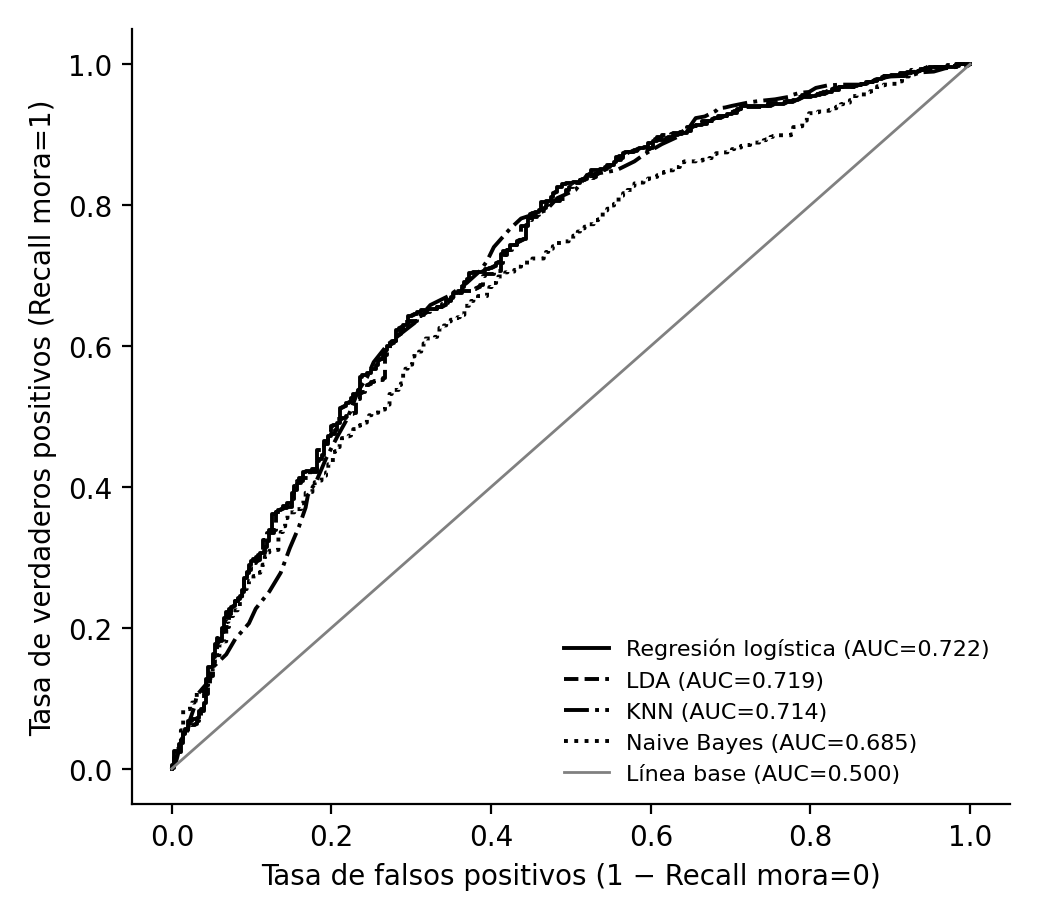
\includegraphics[width=0.85\textwidth]{fig_roc.png}
\caption{Curvas ROC en el conjunto de prueba.}
\label{fig:roc}
\end{figure}

\begin{figure}[H]
\centering
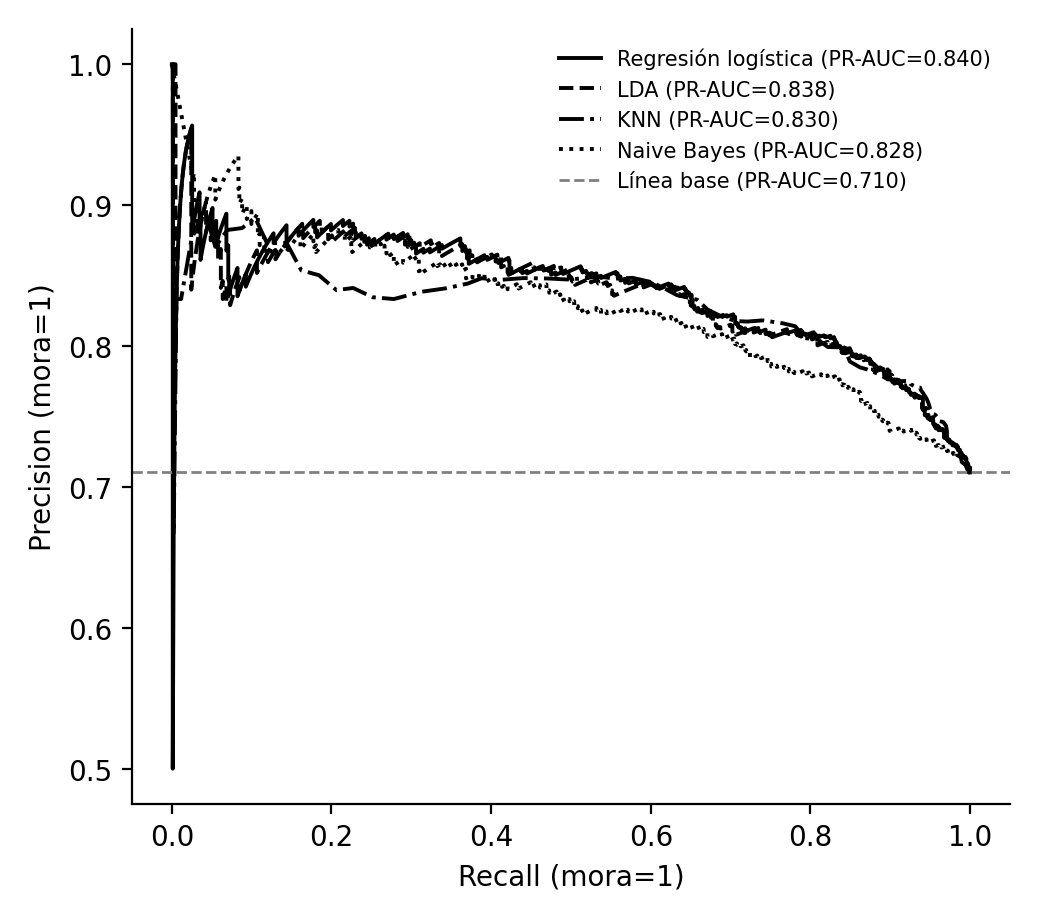
\includegraphics[width=0.85\textwidth]{fig_pr.png}
\caption{Curvas precision--recall en prueba. La línea horizontal es la prevalencia de mora ($\approx$0,71).}
\label{fig:pr}
\end{figure}

Logística, LDA y KNN suben el AUC de 0,5 a $\approx$0,72. Naive Bayes llega a 0,685. Las diferencias entre los tres primeros son menores que la desviación de la validación cruzada, así que no coronamos un único ganador. Un remuestreo bootstrap del conjunto de prueba deja el AUC de la logística entre 0,689 y 0,751, y el de Naive Bayes entre 0,654 y 0,718. Los tres modelos principales se solapan.

Con umbral 0,5 la logística deja escapar 50 morosos de 863 y reconoce apenas al 24,7\% de los buenos pagadores. Con Youden el recall de mora=0 sube a 0,634, a costa de 268 falsos negativos. Cuál conviene depende de cuánto le cueste al banco cada error, y esta base no lo dice.

\section{Sensibilidad a las variables sospechosas}

\begin{table}[H]
\centering
\caption{AUC en prueba según el escenario de variables.}
\label{tab:sens}
\small
\begin{tabular}{@{}lccc@{}}
\toprule
\textbf{Modelo} & \textbf{A. Completo} & \textbf{B. Principal} & \textbf{C. sin score} \\
\midrule
Regresión logística & 0,734 & 0,722 & 0,709 \\
LDA & 0,730 & 0,719 & 0,707 \\
KNN & 0,721 & 0,714 & 0,702 \\
Naive Bayes & 0,692 & 0,685 & 0,677 \\
\bottomrule
\end{tabular}
\end{table}

Incluir \texttt{atraso} y \texttt{clasif\_sbs} sube el AUC unos 0,007 a 0,012, menos que la variación de la CV. Quitar el \texttt{score} baja el AUC a 0,709 en la logística. Nos quedamos con el escenario B: perdemos poco poder predictivo y evitamos variables que podrían medirse después de la mora.

\section{Interpretación preliminar y supuestos}

Usamos los coeficientes de la logística del escenario B (Figura~\ref{fig:coef}) como asociaciones en esta muestra, no como causas. Las variables numéricas están estandarizadas, así que se pueden comparar. En esta base, mayor educación universitaria, más experiencia en el sistema, mayor \texttt{score} y mayor \texttt{nivel\_ahorro} van con menor probabilidad de mora (coeficientes $-$0,49, $-$0,31, $-$0,29 y $-$0,29). Mayor deuda y vivienda propia, frente a alquilada, van con un poco más de mora. La edad casi no aporta. Que estudiar más se asocie a menos mora no significa que estudiar cause el pago: educación, ingreso y empleo van juntos.

\begin{figure}[H]
\centering
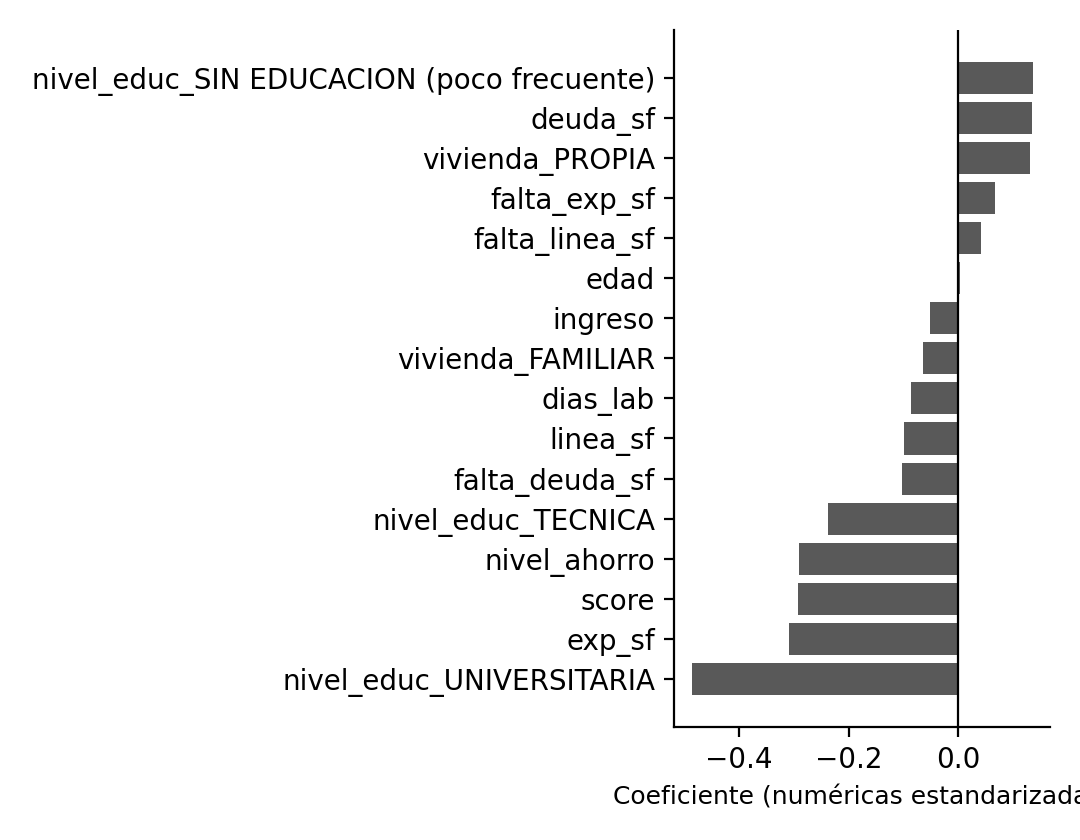
\includegraphics[width=0.88\textwidth]{fig_coeficientes.png}
\caption{Coeficientes de la regresión logística (sin zonas).}
\label{fig:coef}
\end{figure}

Separamos tres tipos de supuestos. Del modelo: \texttt{mora} es binaria, las filas son independientes, la relación es lineal con el \textbf{logit} (no con la probabilidad) y el VIF es bajo. De preprocesamiento: mediana con indicador, duplicados fuera, escenario B. De calidad de los datos: la etiqueta está bien medida y el 71\% de mora no es la prevalencia real del Perú (4\% a 11\% según la SBS). Las probabilidades sirven para ordenar clientes, no para leer riesgo poblacional.

\section{Limitaciones y próximos pasos}

Sin diccionario, la definición de \texttt{mora} y los momentos de cada variable son supuestos. Sin fechas ni identificador de cliente no hay validación temporal ni certeza de que los duplicados sean la misma persona. Para la entrega final, si el curso lo cubre, entra QDA y regularización. También hace falta un costo de cada error para elegir umbral de operación.

\section*{Declaración de uso de inteligencia artificial}

Usamos un modelo de lenguaje como apoyo para código y borradores. El equipo revisó, ajustó y es responsable del contenido. El planteamiento, la base, las variables, los modelos y la lectura de resultados son nuestros.

\section*{Referencias}

\begin{enumerate}[leftmargin=1.6em]
\item Attota, D. C., \& Yarmohammadtoosky, S. (2024). \textit{Optimizing Fintech Marketing: A Comparative Study of Logistic Regression and XGBoost}. Kennesaw State University. arXiv:2412.16333.
\item Calderón Baldeón, L. H. (2021). \textit{BankDefaultAnalysis: Morosidad del Sistema Financiero} [Conjunto de datos]. Kaggle. \url{https://doi.org/10.34740/KAGGLE/DSV/2528417}
\item Superintendencia de Banca, Seguros y AFP del Perú (SBS). (2021). \textit{Clasificación de riesgo crediticio y estadísticas de morosidad del sistema financiero peruano}. \url{https://www.sbs.gob.pe}
\end{enumerate}

\end{document}
